\documentclass[aspectratio=169]{beamer}
\setbeamertemplate{navigation symbols}{}
\usepackage{color,amsmath,comment, subfigure}
\usepackage{booktabs}
\def\vf{\vfill}
\usepackage{url}

\def\imagetop#1{\vtop{\null\hbox{#1}}} %http://tex.stackexchange.com/questions/23521/tabular-vertical-alignment-to-top

%\setbeameroption{show notes}

%%%%%%%%%%%%%%%%%%%%%%%%%%
\title[]{Class 17: Going viral}
\author[]{Matthew J. Salganik}
\institute[]{Sociology 204: Social Networks\\Princeton University}
\date[]{
2/2 Can cascades be predicted?
\vfill

\begin{flushleft}
\vspace{0.6in}

\includegraphics[width=0.1\textwidth]{figures/cc.png}
\end{flushleft}
}

\begin{document}
%%%%%%%%%%%%%%%%%%%%%%%%%%%
\frame{\titlepage}
%%%%%%%%%%%%%%%%%%%%%%%%%%%
\begin{frame}

\begin{figure}
  \centering
  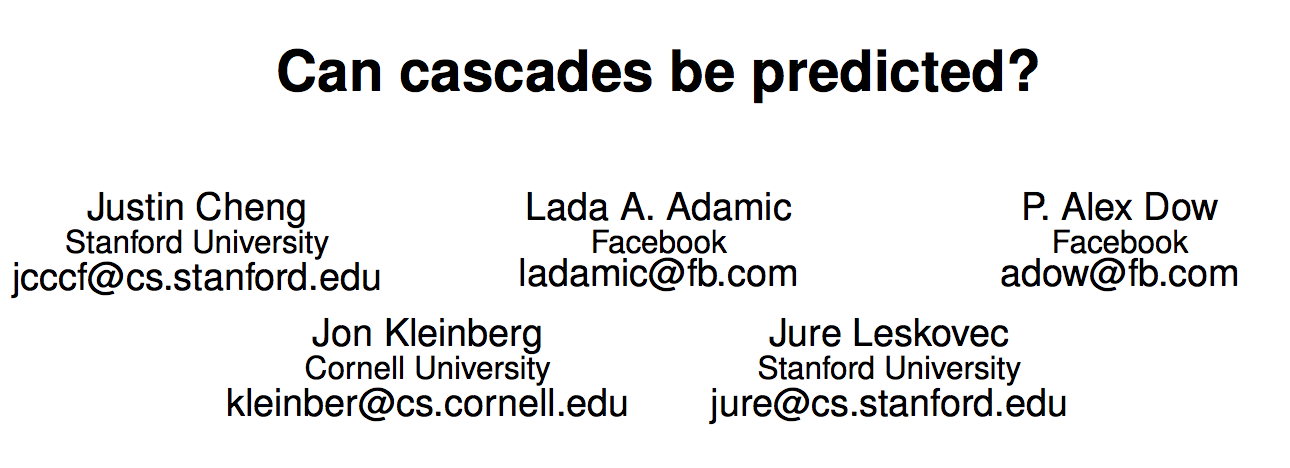
\includegraphics[width=0.9\textwidth]{figures/cheng_cascades_2014_title}
\end{figure}

\end{frame}
%%%%%%%%%%%%%%%%%%%%%
\begin{frame}

\begin{figure}
  \centering
  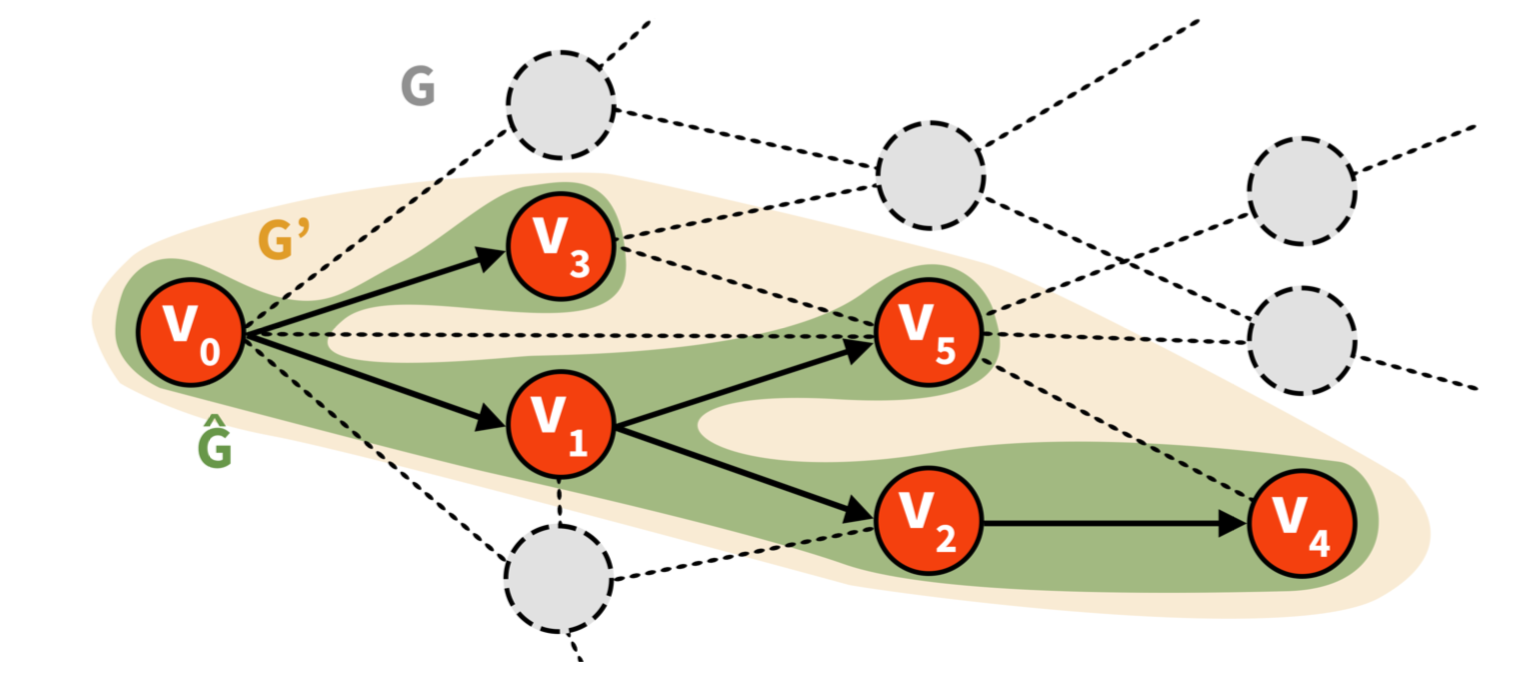
\includegraphics[width=0.9\textwidth]{figures/cheng_cascades_2014_fig1}
\end{figure}

\vfill
Reshare cascades of images on Facebook in June 2013

\end{frame}
%%%%%%%%%%%%%%%%%%%%%
\begin{frame}

Two ways of posting the same question (in this case):
\begin{itemize}
\item Given a cascade that current has size $k$, will grow beyond the median size of $f(k)$?
\item Given a cascade of size $k$, will the cascade double in size and reach at least $2k$ nodes?
\end{itemize}

\end{frame}
%%%%%%%%%%%%%%%%%%%
\begin{frame}

\begin{center}
  \only<1>{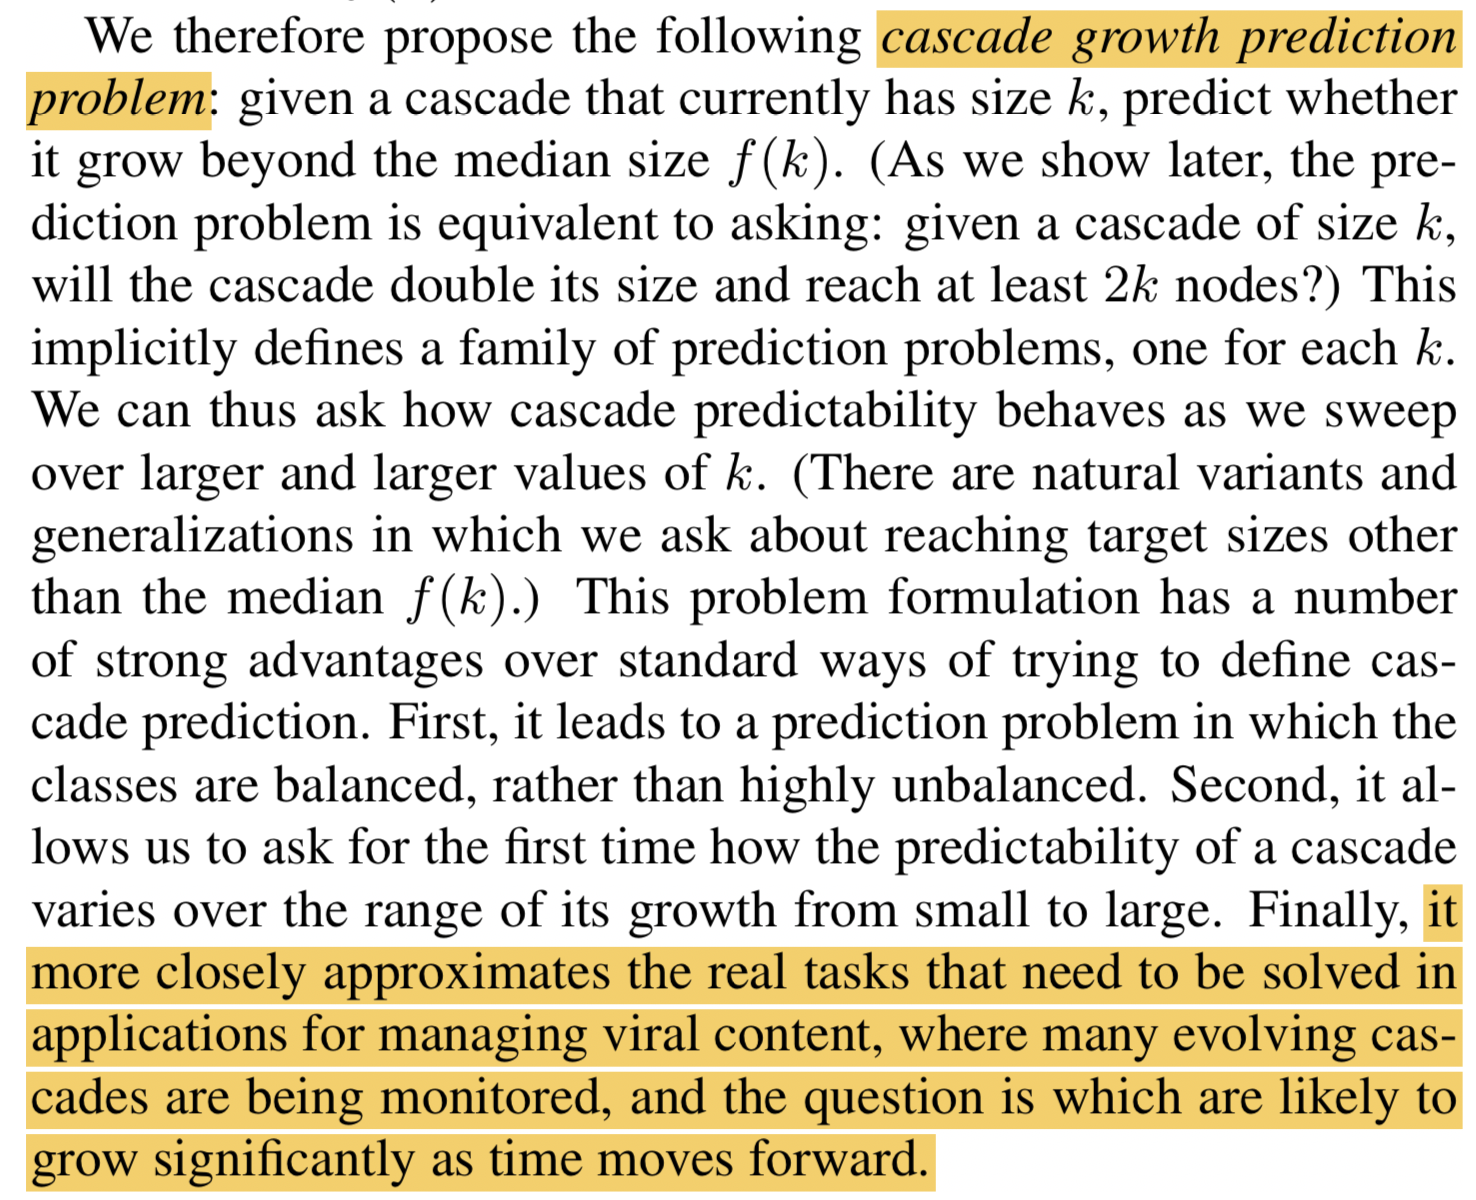
\includegraphics[height=0.9\textheight]{figures/cheng_cascades_2014_problem}}%
  \only<2->{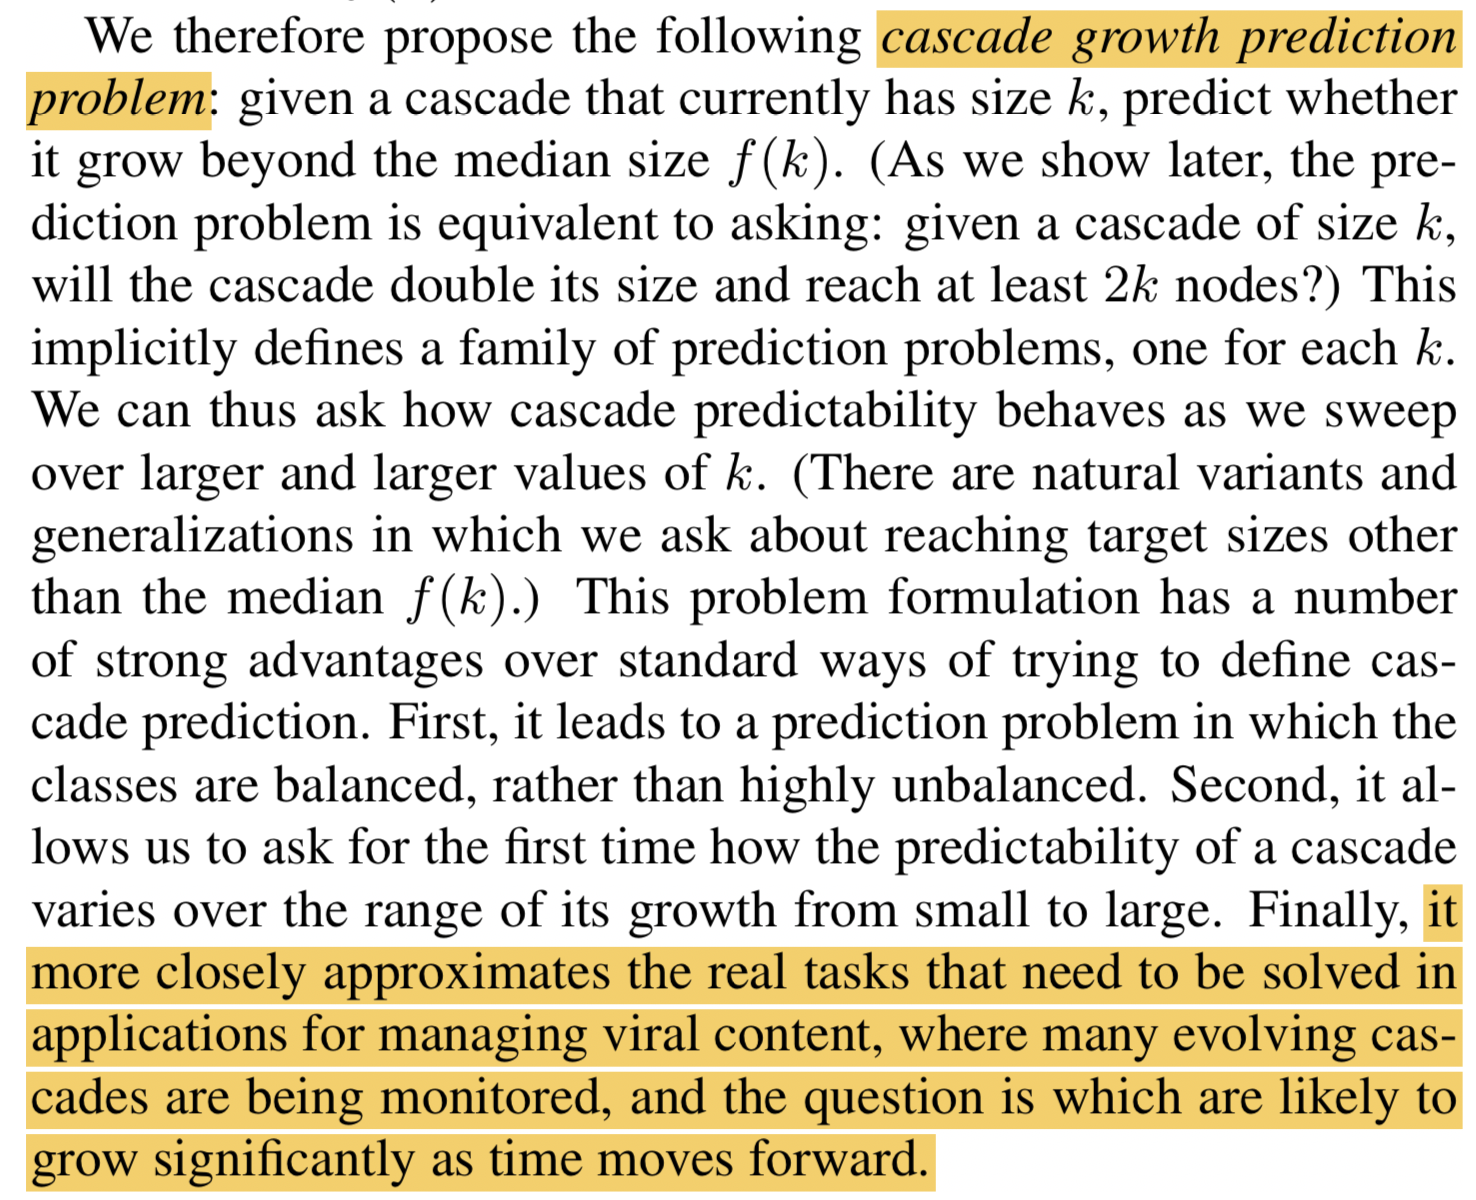
\includegraphics[height=0.5\textheight]{figures/cheng_cascades_2014_problem}}%  
\end{center}

\pause
Why might we need to manage viral content?
\begin{itemize}
\item Amplify virality \pause
\item Check and possible pull things that appear likely to go viral
\end{itemize}

\note{
Scientific and use-based motivation
}

\end{frame}
%%%%%%%%%%%%%%%%%%%
\begin{frame}

\begin{center}
  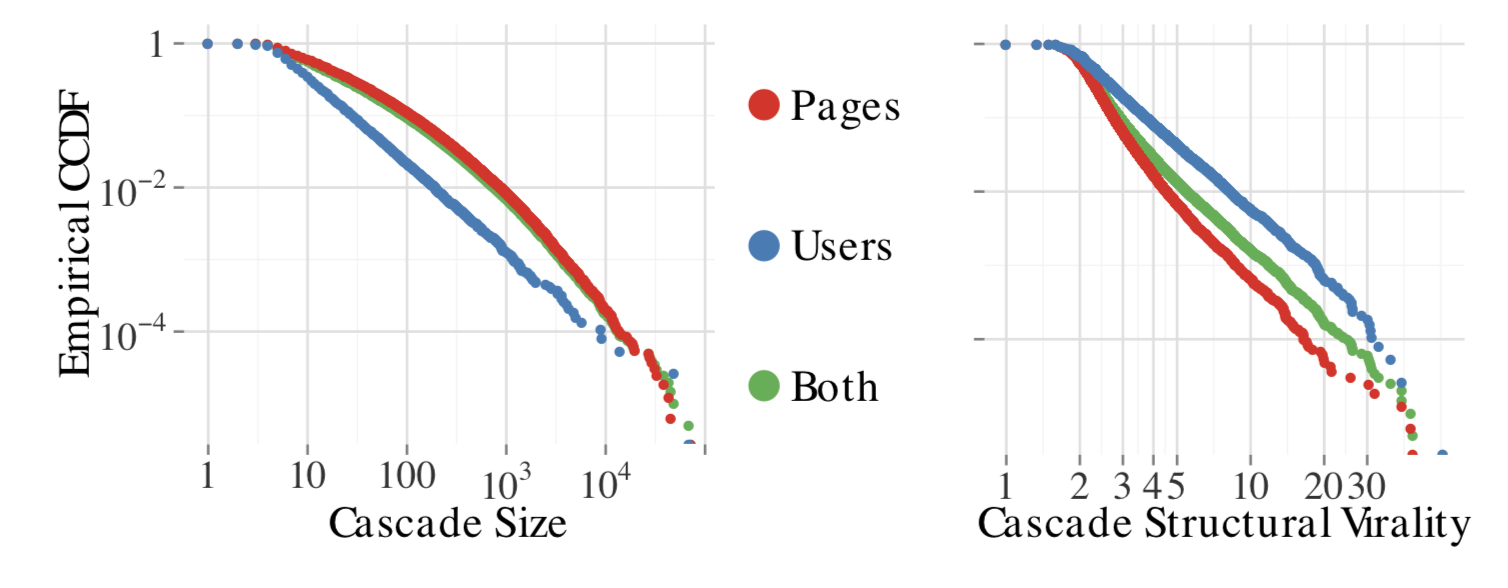
\includegraphics[width=0.9\textwidth]{figures/cheng_cascades_2014_fig2}
\end{center}

Difference between pages (media, celebrities) and users (organic):
\begin{itemize}
\item user cascades are small than page cascades \pause
\item user cascades tend to have higher structural virality
\end{itemize}

\note{
What do cascades look like?}

\end{frame}
%%%%%%%%%%%%%%%%%%%
\begin{frame}

\begin{figure}
  \centering
  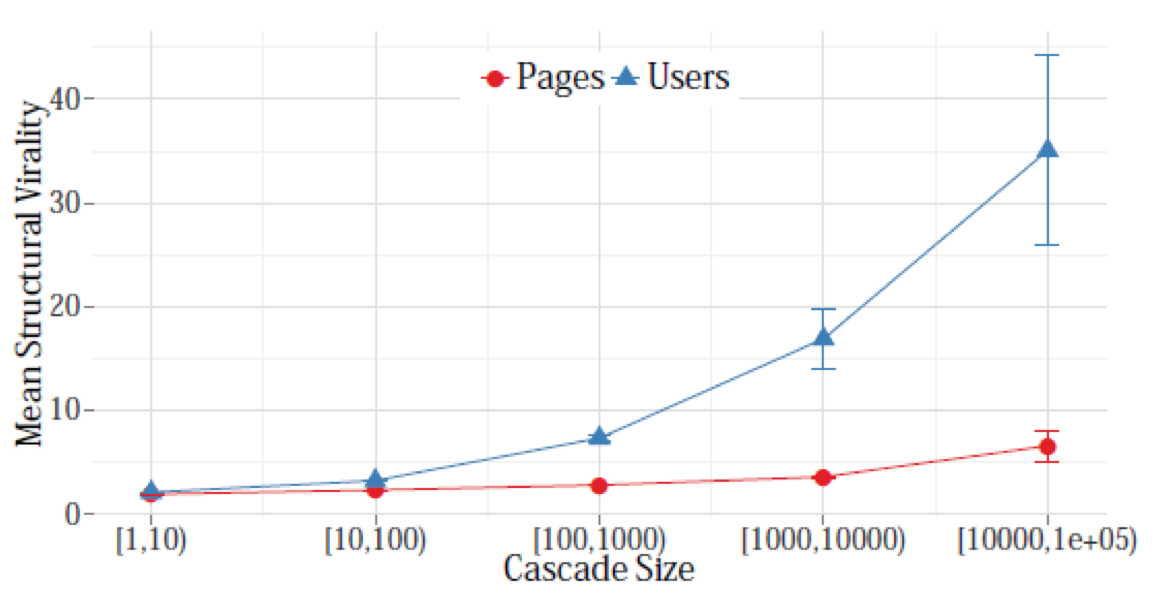
\includegraphics[width=0.6\textwidth]{figures/cheng_cascades_2014_fig8_nocaption}
\end{figure}

\pause

\only<2>{
\begin{figure}
  \centering
  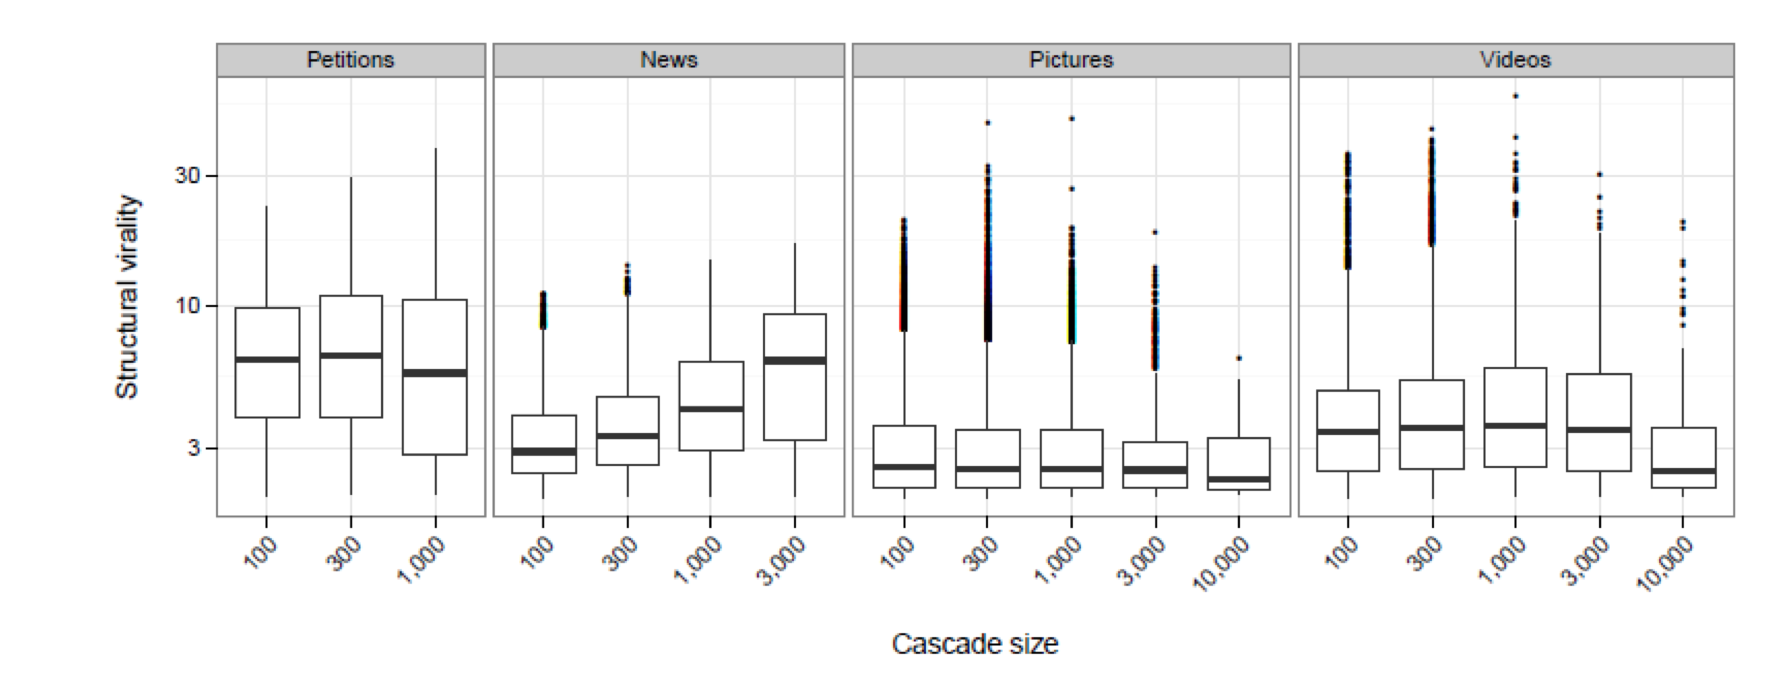
\includegraphics[width=0.6\textwidth]{figures/goel_structural_2016_fig5_nocaption}
\end{figure}
}

\pause
\begin{itemize}
\item For page cascades, there is a weak relationship between size and virallity (similar to Goel et al) \pause
\item For user cascades, there is a strong positive relationship between size and virallity (different to Goel et al)
\end{itemize}

\end{frame}
%%%%%%%%%%%%%%%%%%%
\begin{frame}

Machine learning approach (e.g., COS 424) to predicting if a cascade will double\\
\pause
\begin{figure}
  \centering
  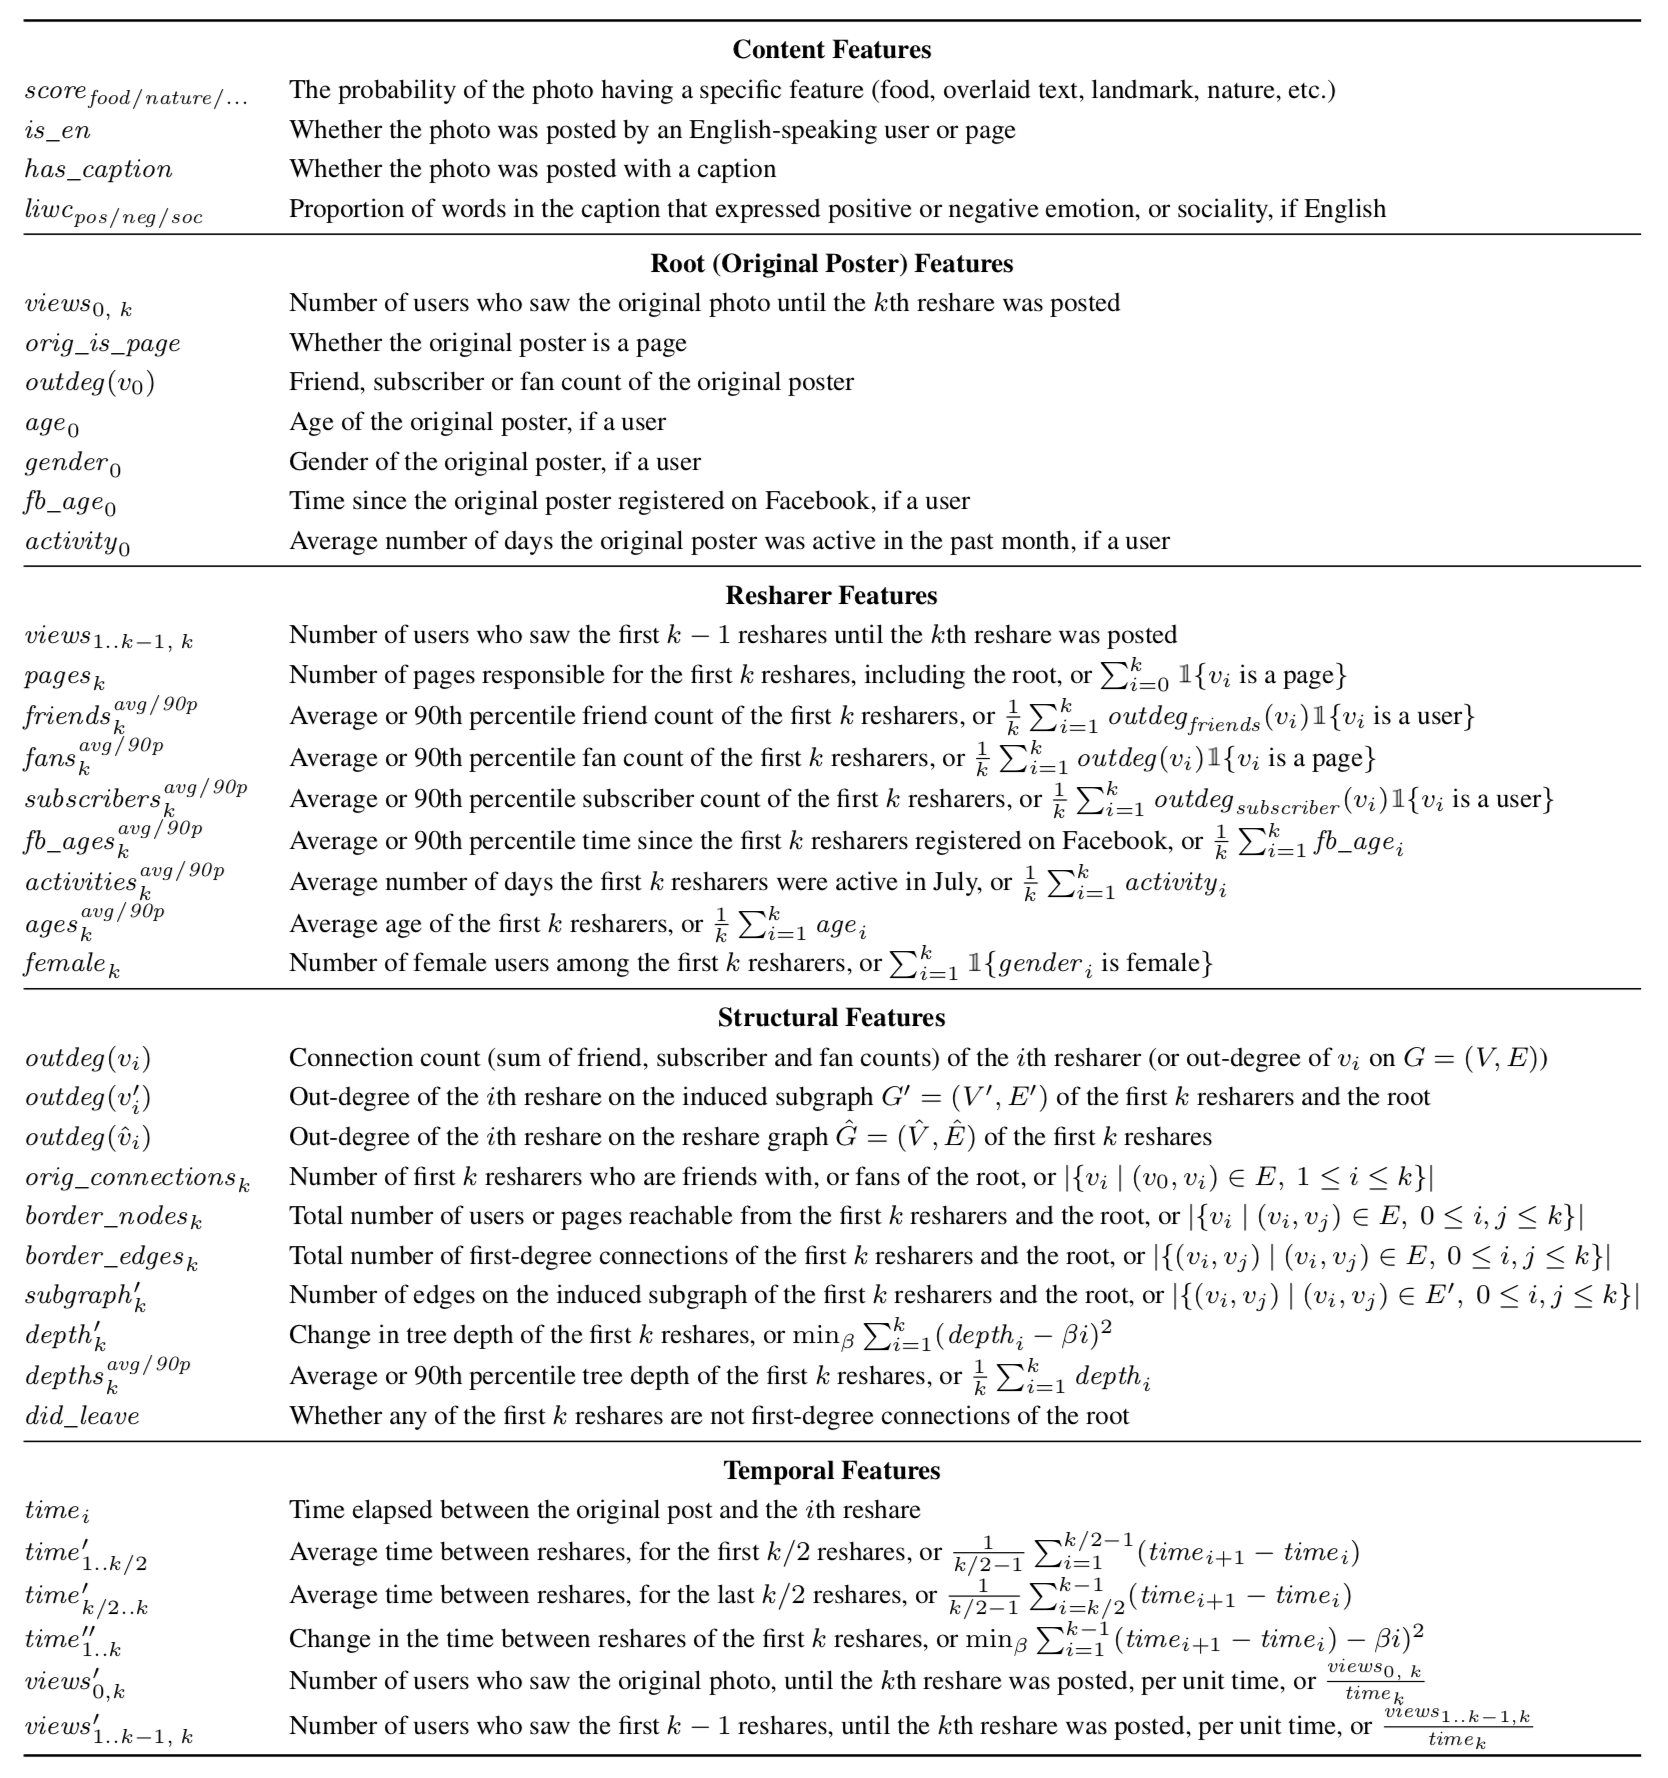
\includegraphics[height=0.85\textheight]{figures/cheng_cascades_2014_tab1.png}
\end{figure}

\note{
5 categories of features:
- Content features
- Original poster
- Resharer features
- Structural features of the cascade
- Temporal
}

\end{frame}
%%%%%%%%%%%%%%%%%%%%%
\begin{frame}

\begin{figure}
  \centering
  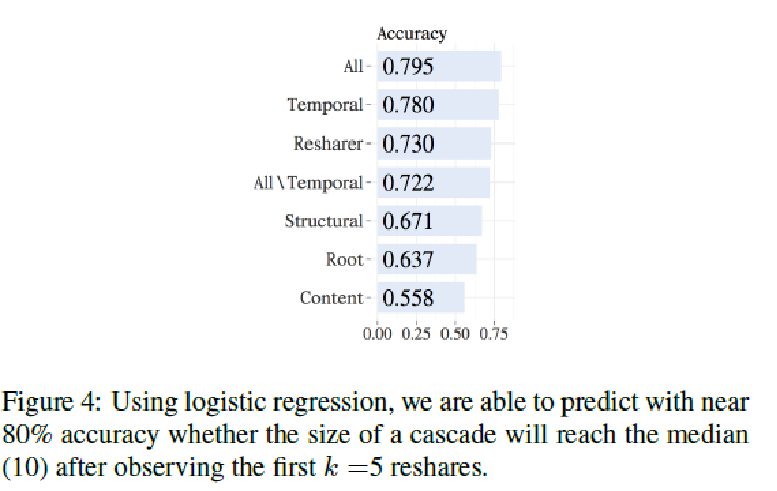
\includegraphics[width=0.7\textwidth]{figures/cheng_cascades_2014_fig4}
\end{figure}

\begin{itemize}
\item Temporal features are most predictive (things that spreading fast are likely to keep spreading) \pause
\item Content features least predictive \pause
\item Temporal features are more predictive than everything else put together
\end{itemize}

\note{
Baseline guessing is 0.5 so content is not a very good set of predictors
}

\end{frame}
%%%%%%%%%%%%%%%%%%%%%
\begin{frame}

\begin{figure}
  \centering
  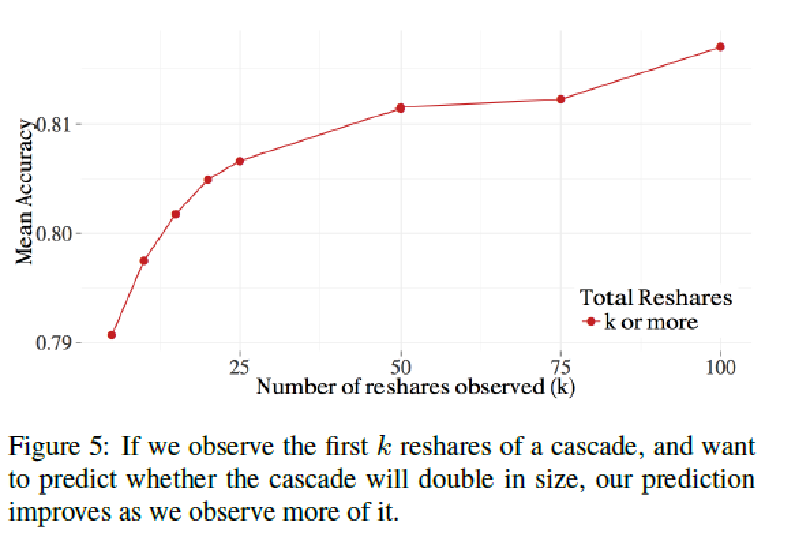
\includegraphics[width=0.9\textwidth]{figures/cheng_cascades_2014_fig5}
\end{figure}

Cascades become slightly more predictable over time

\note{
It is easier to predict if a cascade of size 25 will double than if a cascade of size 10 will double.
}

\end{frame}
%%%%%%%%%%%%%%%%%%%%%
\begin{frame}

\begin{figure}
  \centering
  
\includegraphics[width=0.6\textwidth]{figures/lol_cats_sup_bro}
\end{figure}

\pause 
gini coefficient: 0.787!

\end{frame}
%%%%%%%%%%%%%%%%%%%%
\begin{frame}

\begin{figure}
  \centering
  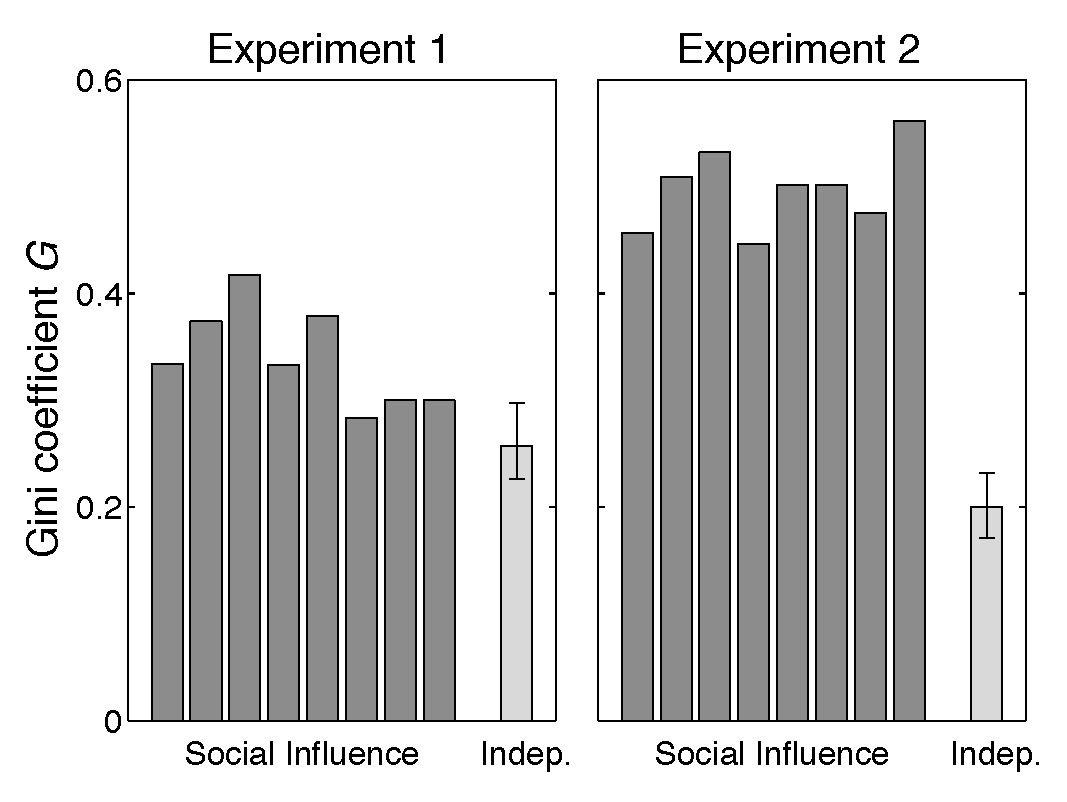
\includegraphics[width=0.7\textwidth]{figures/compare_gini_v1v2_unordered_ci}
\end{figure}

\end{frame}
%%%%%%%%%%%%%%%%%%%%%
\begin{frame}

\begin{figure}
  \centering
  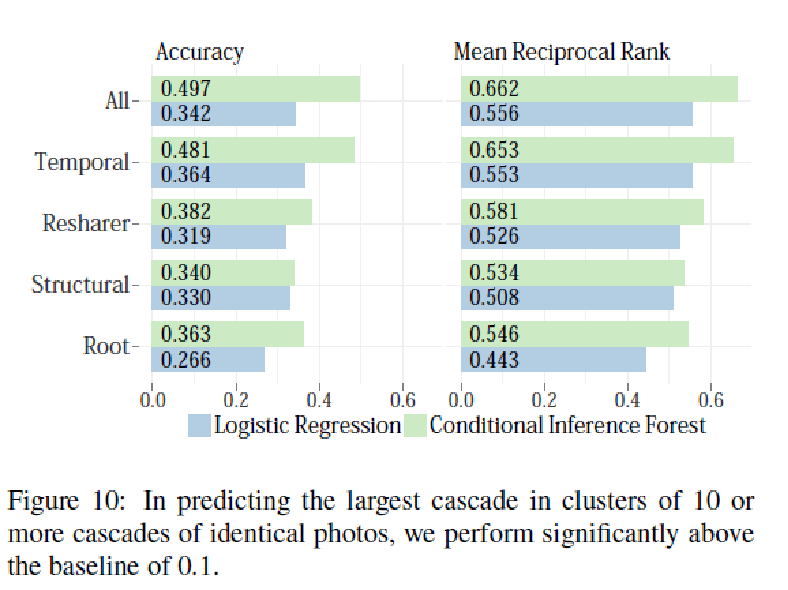
\includegraphics[width=0.7\textwidth]{figures/cheng_cascades_2014_fig10}
\end{figure}

We can somewhat predict which of the identical seeds will spread, if we observe the beginning of each cascade

\note{
But we can predict which of the identical cascades will be more predictable if we watch them begin to spread
}

\end{frame}
%%%%%%%%%%%%%%%%%%%%
\begin{frame}

Summary:
\begin{itemize}
\item asking the right question can be very important in research
\pause
\item almost nothing posted on Twitter and Facebook creates a large cascades
\pause
\item tweets and photos from FB pages show little relationship between structural virality and cascades size; photos from FB users that create large cascades are structurally viral
\pause
\item there are many different ways to ask interesting questions about going viral 
\end{itemize}

\end{frame}
%%%%%%%%%%%%%%%%%%%%
\begin{frame}

What is all this stuff going viral?  

\note{
Is it sunshine and flowers or is it misinformation and hate?

Nobody checked.  I didn't even think to ask.  Now we would.  That turns to our next topic: social media effects on individuals and society.
}
\end{frame}
%%%%%%%%%%%%%%%%%%%%%%%%%%
\begin{frame}

\begin{itemize}
\item Kross, E. et al. (2020). Social media and well-being: Pitfalls, progress, and next steps.  \textit{Trends in Cognitive Science}.
\item Carey, B. (2019). This is your brain off Facebook. \textit{New York Times}.
\item Allcott, H. et al. (2020). The welfare effects of social media. \textit{American Economic Review}.
\item Baym, N.K. et al. (2020). Mindfully scrolling: Rethinking Facebook after time deactived. \textit{Social Media + Society}.
\end{itemize}

\end{frame}
%%%%%%%%%%%%%%%%%%%%%%%%%%

\end{document}
